\section{Adding Time}
\label{section:time}

One of our goals in formalizing the Simple Reactor model is to separate the instantaneous from the time-based aspects.
In previous sections we've built a rigorous model of instantaneous reactors.
In this section, we add the time-based aspects \emph{on top}, i.e. without changing the instantaneous model.
This allows us to model timed reactor networks as a generalization of instantaneous networks, while retaining a separation of concerns.

\subsection{Primitives}
\label{section:time-primitives}

Just as instantaneous reactors defined primitives (ports, state variables, etc.), timed reactor networks are built upon some additional basic notions.

\paragraph{Tags:} In the Reactor model, we use the term \emph{tag} to refer to a logical timestamp. 
Hence, if we want to add a notion of time to our model, we need to formalize tags:

\begin{lstlisting}
def tag := lex ℕ ℕ
\end{lstlisting}

\noindent The type \lstinline{lex} is the Cartesian product, equipped with the lexicographic order.
Thus, the definition above states that \lstinline{tag} is equivalent to $\mathbb{N} \times \mathbb{N}$, and the relation \verb|≤| for \lstinline{tag}s defines a lexicographic order.
This corresponds to the superdense representation of time \cite{dense} mentioned in Section \ref{section:simpel-reactors}.

\subsubsection{Actions as Ports}

In the Instantaneous Reactor model, the entities responsible for carrying values are ports. 
In a time-based model, we additionally want to be able to propagate values through \emph{actions}.
Hence, we generalize the notion of ports and formalize actions as special ports, called \emph{action ports} --- a concept also employed in \cite{marten}.
We will see that this also allows us to drop the formalization of \emph{events} entirely.
In this section we give a rough overview of action ports.
Their details will be covered in Sections \ref{section:timed-network} and \ref{section:timed-exec-model}.

While regular ports have the ability to carry values \emph{across reactors}, this propagation is limited to occur at a fixed logical time.\footnote{
    All ports are cleared after each logical time step (cf. Section \ref{section:execution-model-steps}).
}
With action ports, we want to achieve the inverse goal.
We want values to be propagated between reactions of a single reactor, but \emph{across time}.
As a result, reactions need to be able to specify \emph{when} values should be propagated.
To achieve this, we can exploit the fact that the formalization of instantaneous reactors introduces a generic \emph{value} type \lstinline{υ}, on which virtually all components of the model are dependent.
That is, instantaneous reactors work the same no matter which specific type \lstinline{υ} is.
Thus, in time-based reactor networks, we give \lstinline{υ} a structure that allows reactions to add tags to their outputs.
We call this structure a \emph{timed port assignment} (TPA).

\paragraph{TPAs:}

A TPA consists of a finite number of tag-value pairs:

\begin{lstlisting}
variables (υ : Type*) [decidable_eq υ] 
def tpa := finset (tag × option υ)
\end{lstlisting}

\noindent As in Section \ref{section:formal-inst-reactors}, we define the underlying data \emph{values} by means of an equatable dependent type parameter \lstinline{υ}. 
The tags in a TPA specify \emph{when} actions, which carry given values, should be scheduled.
Since reactions can schedule multiple actions per execution, TPAs are not just a single tag-value pair, but a collection of them.

While the definition of TPAs is well-suited for action ports, we must consider their interaction with regular ports.
Since we make no distinction in the kinds of values that are passed to different kinds of ports\footnote{We \emph{can't}, without changing the formalization of instantaneous reactors.}, action ports and regular ports both carry TPAs.
We may therefore need to define what it means for a regular port (and by extension a reaction) to receive a TPA.
Fortunately the GIGO principle can resolve this issue:
We declare that all regular ports and reaction bodies must only receive TPAs that contain exactly one tag-value pair where the tag is the current logical time.
Otherwise, no guarantees about a network's behavior are made.
The ``instantaneous value'' of such a TPA is then the value contained in the TPA's only tag-value pair.

\subsection{Timed Networks}
\label{section:timed-network}

To understand the behavior of TPAs more clearly, we first need to define action ports more rigorously.
The only difference between regular ports and action ports is in how we treat them in timed reactor networks:

\lstset{numbers=left, xleftmargin=1.5em}
\begin{lstlisting}
structure timed.network :=
  (σ : inst.network (tpa υ))
  (time : tag)
  (event_queue : list tag)
  (actions : finset action_edge)
  (well_formed : actions.are_well_formed_for σ)
\end{lstlisting}
\lstset{numbers=none, xleftmargin=0em}

\noindent A \lstinline{timed.network} is an extension on an \lstinline{inst.network}.
We define the underlying network to use \lstinline{tpa}s for its values (Line 2).
That is, the data values in the instantaneous world are of type \lstinline{(tpa υ)}, while the data values in the time-based world are of type \lstinline{υ}.
Lines 3 and 4 add properties that will be explained in Section \ref{section:timed-exec-model}.
The properties concerning action ports are on Lines 5 and 6.

\subsubsection{Action Edges}

Reactors come with \emph{output} and \emph{input} ports, which receive values from reactions and propagate values into reactions respectively.
We generalize this notion to action ports and talk about \emph{output action ports} (OAP) and \emph{input action ports} (IAP).
OAPs receive the TPAs produced by reactions and IAPs propagate values back into reactions.
We can connect OAPs and IAPs using special edges:

\begin{lstlisting}
structure timed.network.action_edge := 
  (oap : port.id)
  (iap : port.id)
\end{lstlisting}

\noindent Thus, everything that is an \emph{action} in the Simple Reactor model is now represented by an OAP, an IAP, and an edge between them.\footnote{
    We will see below that we sometimes need multiple OAPs per action.
}
If a reaction wants to be able to schedule a specific action, it needs to declare a corresponding OAP as its antidependency.
If a reaction wants to be able to receive values from an action, it needs to declare that action's IAP as a dependency.

While this system works well at first glance, we need to consider the following scenario:
What if multiple reactions want to schedule the same action?
Since output ports may have multiple inputs, i.e. be an antidependency for multiple reactions, we can connect multiple reactions to the same OAP.
This leads to the problem that, if two reactions schedule the same action during the same round of execution, they both write to the same OAP.
Thus, one of their TPAs will override the other.
What we would want is for their TPAs to be merged into a single TPA.
But to achieve this we would have to adjust the implementation of instantaneous reactors.
Hence, we take a different approach --- we allow each action to have multiple OAPs.
Each reaction that wants to schedule an action can then connect to its own unique OAP, so no overriding occurs.
Figure \ref{fig:timed-reactor} shows an example of a reactor that contains an action with multiple connected reactions (and therefore multiple OAPs), as well as a reaction that schedules multiple different actions.

\begin{figure}[h]
\centering
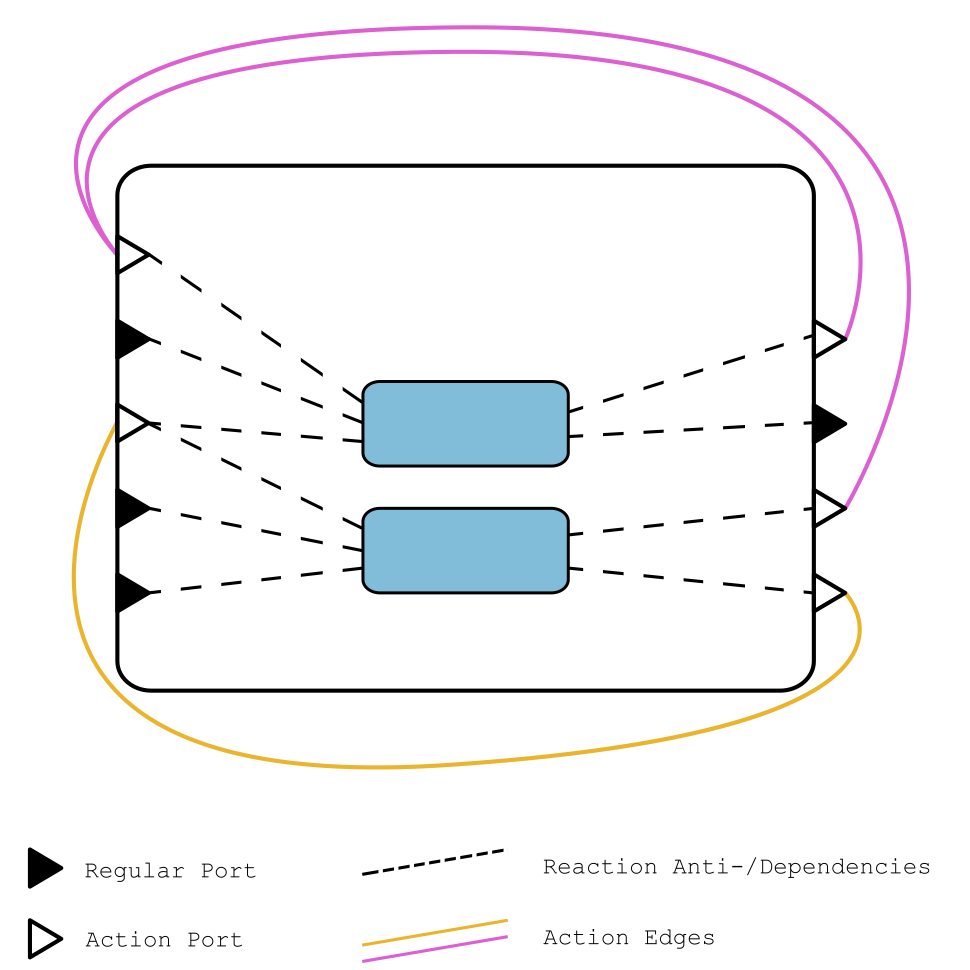
\includegraphics[width=0.66\textwidth]{timed-reactor}
\caption{Reactor with two actions}
\label{fig:timed-reactor}
\end{figure}
  
\subsubsection{Well-Formedness}
 
Modeling actions as ports and edges only works subject to some constraints.
These constraints are enforced by \lstinline{timed.network.well_formed} (Line 6 above):

\begin{lstlisting}
def finset.are_well_formed_for 
  (es : finset action_edge) (σ : inst.network (tpa υ)) :=
    es.are_many_to_one ∧ 
    es.are_local ∧
    es.have_unique_source_in σ ∧ 
    es.are_functionally_unique_in σ ∧
    es.are_separate_from σ
\end{lstlisting}

\noindent We go through these constraints in order:

\begin{enumerate}[leftmargin=14pt]
\item Each action has exactly one IAP, and OAPs can belong to only one action. Thus, OAPs cannot be connected to multiple IAPs:
\begin{lstlisting}
def finset.are_many_to_one (es : finset action_edge) :=
  ∀ e e' : action_edge, e ∈ es → e' ∈ es →
    e.oap = e'.oap → e = e'
\end{lstlisting}
\item Actions are local to a single reactor. Hence, action edges must begin and end in the same reactor:
\begin{lstlisting}
def finset.are_local (es : finset action_edge) :=
  ∀ e : action_edge, e ∈ es → 
    e.oap.rtr = e.iap.rtr
\end{lstlisting}
\item To avoid overriding of TPAs (as previously explained), OAPs may be connected to at most one reaction.
The expression \lstinline{(σ.η.deps r role.output)} returns the output-dependencies of a reaction \lstinline{r}:
\begin{lstlisting}
def finset.have_unique_source_in 
  (es : finset action_edge) (σ : inst.network (tpa υ)) :=
    ∀ (e : action_edge) (r r' : reaction.id), e ∈ es → 
      (e.oap ∈ σ.η.deps r role.output) → 
      (e.oap ∈ σ.η.deps r' role.output) → 
      r = r'
\end{lstlisting}
\item A single reaction cannot use multiple OAPs for scheduling the same action. 
That is, if a reaction connects to two distinct OAPs, they cannot connect to the same IAP.
We make this restriction, because the execution of a timed reactor network will require us to merge TPAs.
The order in which we perform merges is based on the priorities of OAPs.
An OAP's priority is inherited from the reaction it is connected to.
Hence, this restriction is necessary to keep OAPs' priorities unique, thereby allowing us to impose a total order on them, which allows us to retain determinism when merging TPAs:

\break

\begin{lstlisting}
def finset.are_functionally_unique_in 
  (es : finset action_edge) (σ : inst.network (tpa υ)) :=
    ∀ (e e' : action_edge) (r : reaction.id), 
      e ∈ es → e' ∈ es → 
      (e.oap ∈ σ.η.deps r role.output) → 
      (e'.oap ∈ σ.η.deps r role.output) → 
      e.iap = e'.iap → 
      e.oap = e'.oap
\end{lstlisting}
\item While action ports are \emph{just ports}, they should not also take on the role of regular untimed ports.
Hence, it must be ensured that no ``regular network edges'' are attached to them:
\begin{lstlisting}
def finset.are_separate_from 
  (es : finset action_edge) (σ : inst.network (tpa υ)) :=
    ∀ (ae : action_edge) (ne : inst.network.graph.edge), 
      ae ∈ es → ne ∈ σ.η.edges → 
      ae.iap ≠ ne.dst ∧ ae.oap ≠ ne.src
\end{lstlisting}
\end{enumerate}

\noindent Giving action ports their own separate edges and imposing these five restrictions, allows us to model actions as a generalization ports.

\subsection{Execution Model}
\label{section:timed-exec-model}

Just as the definition of timed reactor networks builds heavily on that of instantaneous reactor networks, so does the execution model.
Time-based execution can be modeled as a sequence of instantaneous executions. 
To achieve this, we require two things: a global logical time and an event queue.
We've already added these components in our definition of \lstinline{timed.network} above:

\begin{itemize}
  \item \lstinline{time} is the tag for the current logical time.
  \item \lstinline{event_queue} is an ordered list of tags, that indicates at which logical times the next instantaneous executions need to take place.
  In our Simple Reactor model, a tag can only be added to this queue as the result of scheduling an action for that tag.
  Note that, while the event queue in the Simple Reactor model has explicit \emph{event} objects in its event queue, this formalization only queues \emph{tags}.
  Explicit event objects are not used at all in this formalization.
\end{itemize}

\noindent Execution of a timed reactor network progresses as follows.
As long as there are events in the event queue, we execute an instantaneous version of the network at the tag of the next event.
The IAPs in this network must contain the values specified by the actions scheduled for this tag.
Upon completion, integrate the actions scheduled during the instantaneous execution into the timed network and advance the current logical time.

\noindent We formalize this with the following implementation.\footnote{For a discussion of why we formalize by implementation, cf. Section \ref{section:classical-vs-constructive}.}
For every tag $T$ in a timed reactor network's event queue:

\begin{enumerate}
  \item If the event queue is empty, complete execution. Otherwise:
  \item Merge all TPAs from all OAPs into their respective IAPs.
  \item Construct an instantaneous reactor network for the current tag $T$, by removing all tag-value pairs with a tag $\ne T$ from all IAPs' TPAs.
  \item Run the instantaneous network as formalized in Section \ref{section:execution-model}, but clear all regular ports upon completion.
  \item Build a timed network from the result of Step 4:
  \begin{enumerate}
    \item Restore the TPAs in the IAPs to the state from before Step 3.
    \item Set the network's \lstinline{time} to $T$.
    \item For every tag that appears in the executed network's OAPs' TPAs, add it to the existing event queue.
    Then sort the event queue in increasing order (earlier tags preceding later tags).
  \end{enumerate}
  \item Repeat this procedure from Step 1, using the timed network from Step 5 for further execution.
\end{enumerate}

\noindent There are again a variety of small steps required to realize such an algorithm:

\begin{figure}[h]
\centering
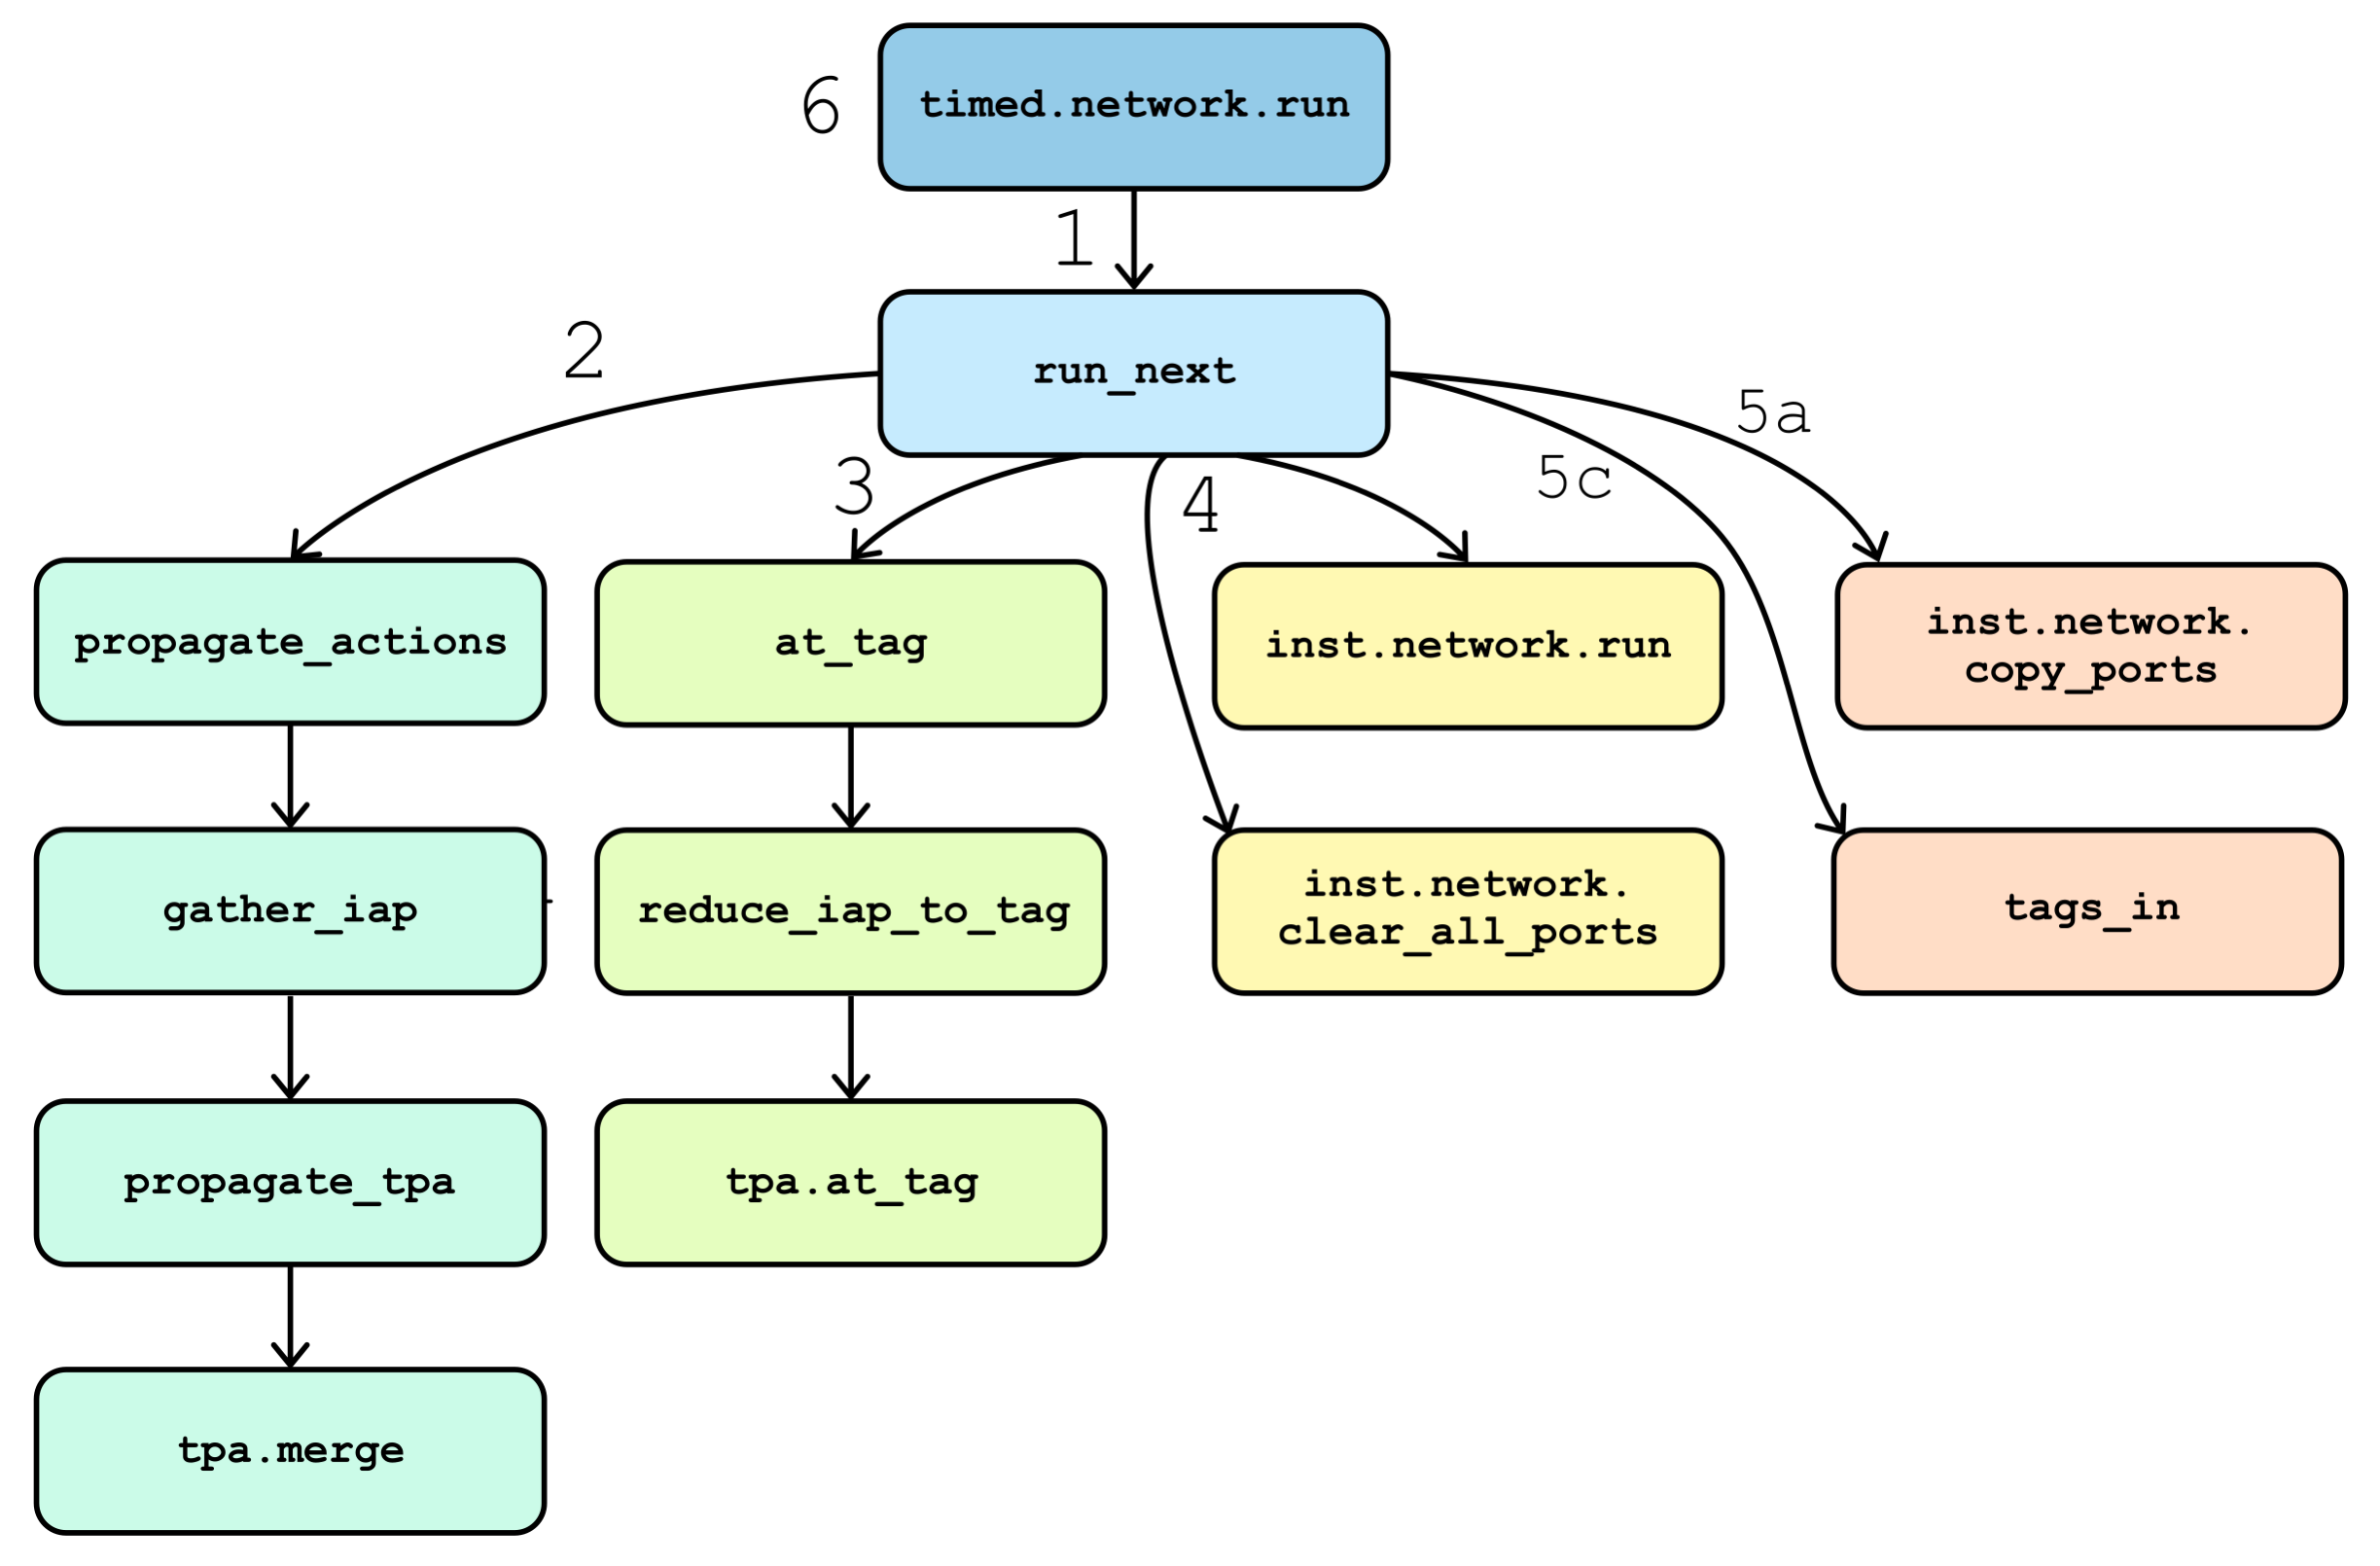
\includegraphics[width=0.9\columnwidth]{timed-exec-steps}
\caption{Functions in the execution of timed reactor networks}
\label{fig:timed-exec-steps}
\end{figure}

\noindent As we show no proofs about timed networks in this thesis, we omit any details about these functions.
Instead, we only consider one important detail about \lstinline{timed.network.run}, namely that it doesn't exist.
We can see why, by examining the core function in the implementation of timed network execution: \lstinline{run_next}.
This function gets the next tag in the event queue and runs the network \emph{only for that tag}:

\begin{lstlisting}
def run_next (τ : timed.network υ)
  (fₚ : prec_func (tpa υ)) (tₚ : topo_func (tpa υ)) : 
  timed.network :=
    match τ.event_queue with 
      | [] := τ
      | hd :: tl := ... -- run `hd`
    end
\end{lstlisting}

\noindent The responsibility of \lstinline{timed.network.run} would then be to implement Step 6 of the execution model.
That is, take whatever \lstinline{run_next} returned and feed it back into \lstinline{run_next}.
As it turns out, directly implementing this step in Lean is impossible. 
We cover the underlying issue in the following section. 

\subsubsection{Infinite Recursion}
\label{section:recursion}

The reason why we cannot implement Step 6 is that it causes potentially infinite recursion.
By ``repeating the procedure from Step 1'' and beginning each iteration \emph{with a new timed network}, we can mutate the event queue on every iteration.
In consequence, we can repopulate it each time, thus causing an infinite number of iterations.
As a minimal example, consider the following timed reactor network:


\begin{figure}[h]
\centering
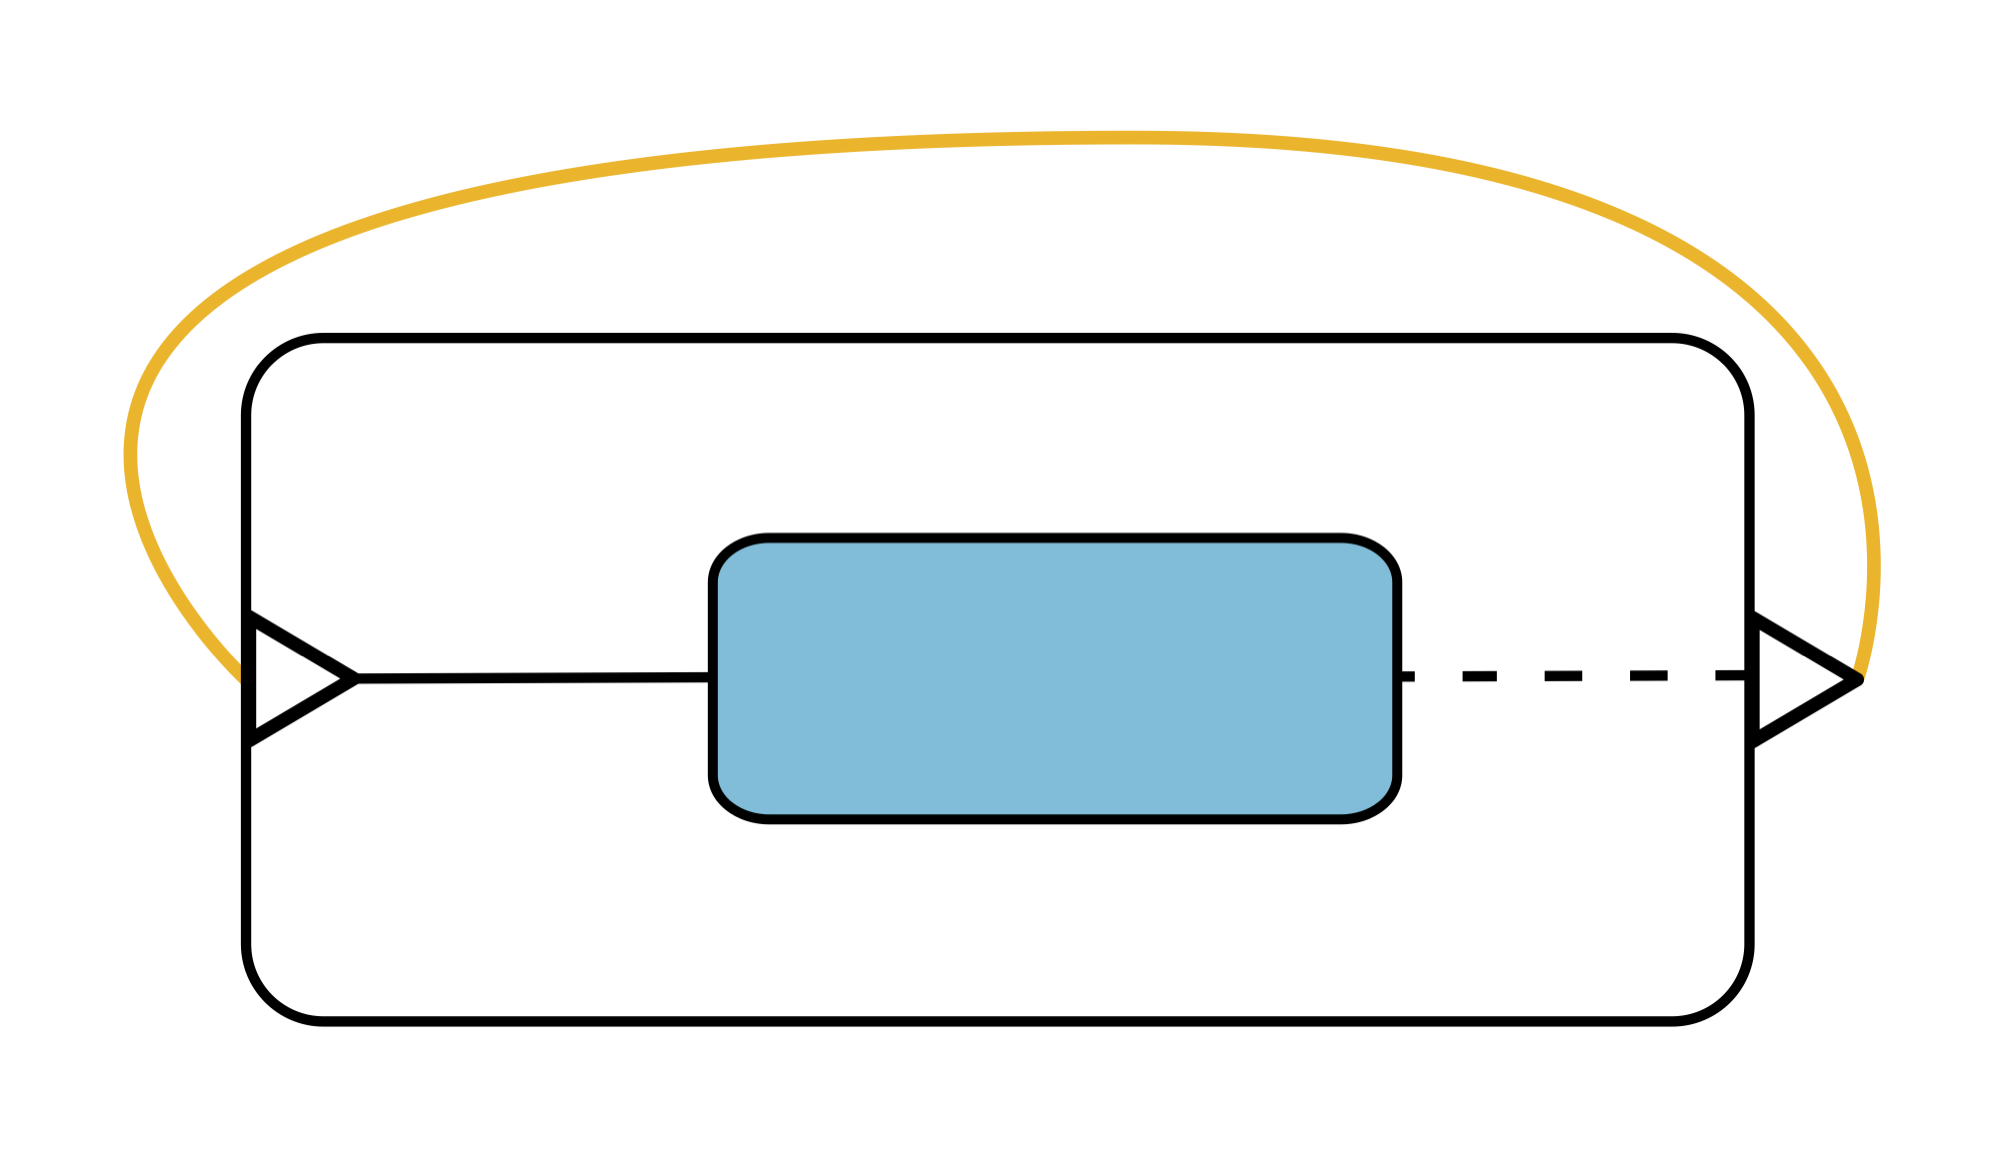
\includegraphics[width=0.5\columnwidth]{infinite-recursor}
\caption{Indefinitely executing timed reactor network}
\end{figure}

\noindent If we assume that the reaction schedules an action every time it executes, it will keep triggering itself, and hence sustain execution indefinitely.

\paragraph{Recursion in Lean:}

While infinite recursion can be trivially implemented in most programming languages, Lean explicitly forbids it.
In fact, recursion is already ruled out by the typed lambda calculus, where the type restrictions for valid terms make it impossible to define recursive functions.
Thus, in Lean, any recursive function definition is rewritten into a valid term by the compiler. 
This is only possible, when the recursively defined function provably terminates.\footnote{
  There technically is a way to define infinite recursion in Lean --- via \verb|meta| functions. 
  These aren't properly checked by Lean and hence allow us to prove \verb|false|.
}
In certain cases, Lean can prove this fact for us, so we don't need to make it explicit.
Take as an example this inductively defined function over lists:

\begin{lstlisting}
def list_sum : list ℕ → ℕ
  | [] := 0
  | (hd :: tl) := hd + list_sum tl
\end{lstlisting}

\noindent For this function, Lean can prove to itself that:

\begin{enumerate}
  \item Every recursive call takes as argument a list that is smaller than the one received by the enclosing function context.
  \item There's a smallest list (the empty list) whose definition for this function is non-recursive.
\end{enumerate}

\noindent Hence, any call to this function can only recurse finitely many times.
When Lean cannot infer that a recursive call is ``decreasing'', we have to implement the recursion manually by means of the well-founded recursion theorem.\footnote{
  For this, Lean provides definitions like \lstinline{well_founded.recursion} and \lstinline{well_founded.fix}.
}
This mechanism allows us to explicitly prove the properties that Lean could infer for the function above.
Since the execution of timed reactor networks can be inherently non-terminating, we cannot prove such properties and are forced to find a different approach for modeling indefinite sequential computation.
We mention a possible solution to this problem in Section \ref{section:future}.
